%% INNOVSAIL template 2020 (org. from voilenav crew)

\documentclass[10pt,a4paper,twocolumn]{article}

% Document packages
\usepackage{amsmath}
\usepackage{amsfonts}
\usepackage{amssymb}
\usepackage{times}
\usepackage{graphicx}
\usepackage{abstract}
\usepackage{fancyhdr}
\usepackage[absolute]{textpos}
\usepackage{booktabs}
\usepackage{url}
\usepackage{algpseudocode}
\usepackage{algorithm}

% Page and style setup
\usepackage[a4paper,top=25mm,bottom=25mm,left=17mm,right=17mm,includefoot]{geometry} 
\usepackage{titlesec}
\usepackage{titlesec}
\usepackage{titling}
\titleformat*{\section}{\bfseries}
\titleformat*{\subsection}{\normalsize}
\titleformat*{\subsubsection}{\normalsize}
\setlength\parindent{0pt}
\setlength{\parskip}{10pt}
\titlespacing*{\section}{0pt}{4pt}{0pt}
\titlespacing*{\subsection}{0pt}{2pt}{0pt}
\titlespacing*{\subsubsection}{0pt}{0pt}{0pt}
\titlespacing*{\paragraph}{0pt}{0pt}{0pt}
\setlength{\headheight}{0pt}
\setlength{\headsep}{0pt}
\setlength{\footskip}{0pt}
\pagestyle{plain}
\renewcommand{\refname}{\protect \normalsize REFERENCES}
\newcommand{\makeauthor}[3]{\normalsize{\textbf{#1}, #2, #3.}\\}

% Nomenclature
\usepackage{nomencl}
\renewcommand{\nomname}{NOTATION}
\makenomenclature

% Abstract
\renewcommand{\abstracttextfont}{\normalsize}
\renewcommand{\abstractname}{}

%--------------------------------------------------------
\begin{document}
\bibliographystyle{plain}
%--------------------------------------------------------
\pagestyle{empty}
\fancyfoot{}
\fancyhead{}

%*********************************************************
%****************  START ARTICLE  ************************
%*********************************************************


%******** TITLE and AUTHORS *****************************


\twocolumn[
	\begin{onecolabstract}
\noindent \Large{\textbf{REPLICATING COMPUTATIONAL OUTPUTS OF RANS-CFD USING MACHINE LEARNING}}\\ \vspace{-0.4 cm}

\makeauthor{N. van der Kolk}{Blue Wasp, Netherlands}{nicovanderkolk@gmail.com}
\makeauthor{B. Freeman}{Lakes Software, Canada}{brian.freeman@weblakes.com}


\vspace{-1.2 cm}\begin{abstract} \noindent 
Reynolds-averaged Navier Stokes computational fluid dynamics (RANS-CFD) packages are often used during the development of performance predictions for commercial ships, requiring intensive computational resources and complex software to generate results. Individual adjustments to parameters require discrete processing that may take hours to process. To expedite results under different hull designs, machine learning models were trained on RANS-CFD outputs to reproduce responses to different input values. The model successfully reproduced the RANS-CFD results with over 98\% accuracy for 60 different hull variations and allowed for rapid estimation of results based on component force inputs. As a result, the different hulls can be quickly evaluated under different input conditions.
\end{abstract}

    \vspace{0.1 cm}
\end{onecolabstract}]

%*****************************************************************************

\section*{NOMENCLATURE}

\begin{tabular}{lll}
Symbol  &	Definition 			&(unit)\\
$\beta$		&	Leeway &(deg)\\
$\phi$    &	Heel angle 	&(deg)\\
Fn	&	Froud number&(unitless)\\
\end{tabular}

\section{INTRODUCTION}
Reynolds-averaged Navier Stokes computational fluid dynamics (RANS-CFD) and other numerical modelling packages are often used during the development of performance predictions for commercial ships to estimate sailing performance \cite{Tezdogan2015}. These methods require intensive computational resources and complex software to generate results, thereby limiting the number of scenarios, hull variations, and operating conditions a specific design can be evaluated under. Performance expectations are essential in new ship design as well as for modifications to existing hulls in order to improve safety and energy efficiency   by estimating power requirements during underway and calm water conditions.

\section{BACKGROUND}

\subsection{Modeling ship performance using RANS-CFD}

\begin{figure}[]
\centering
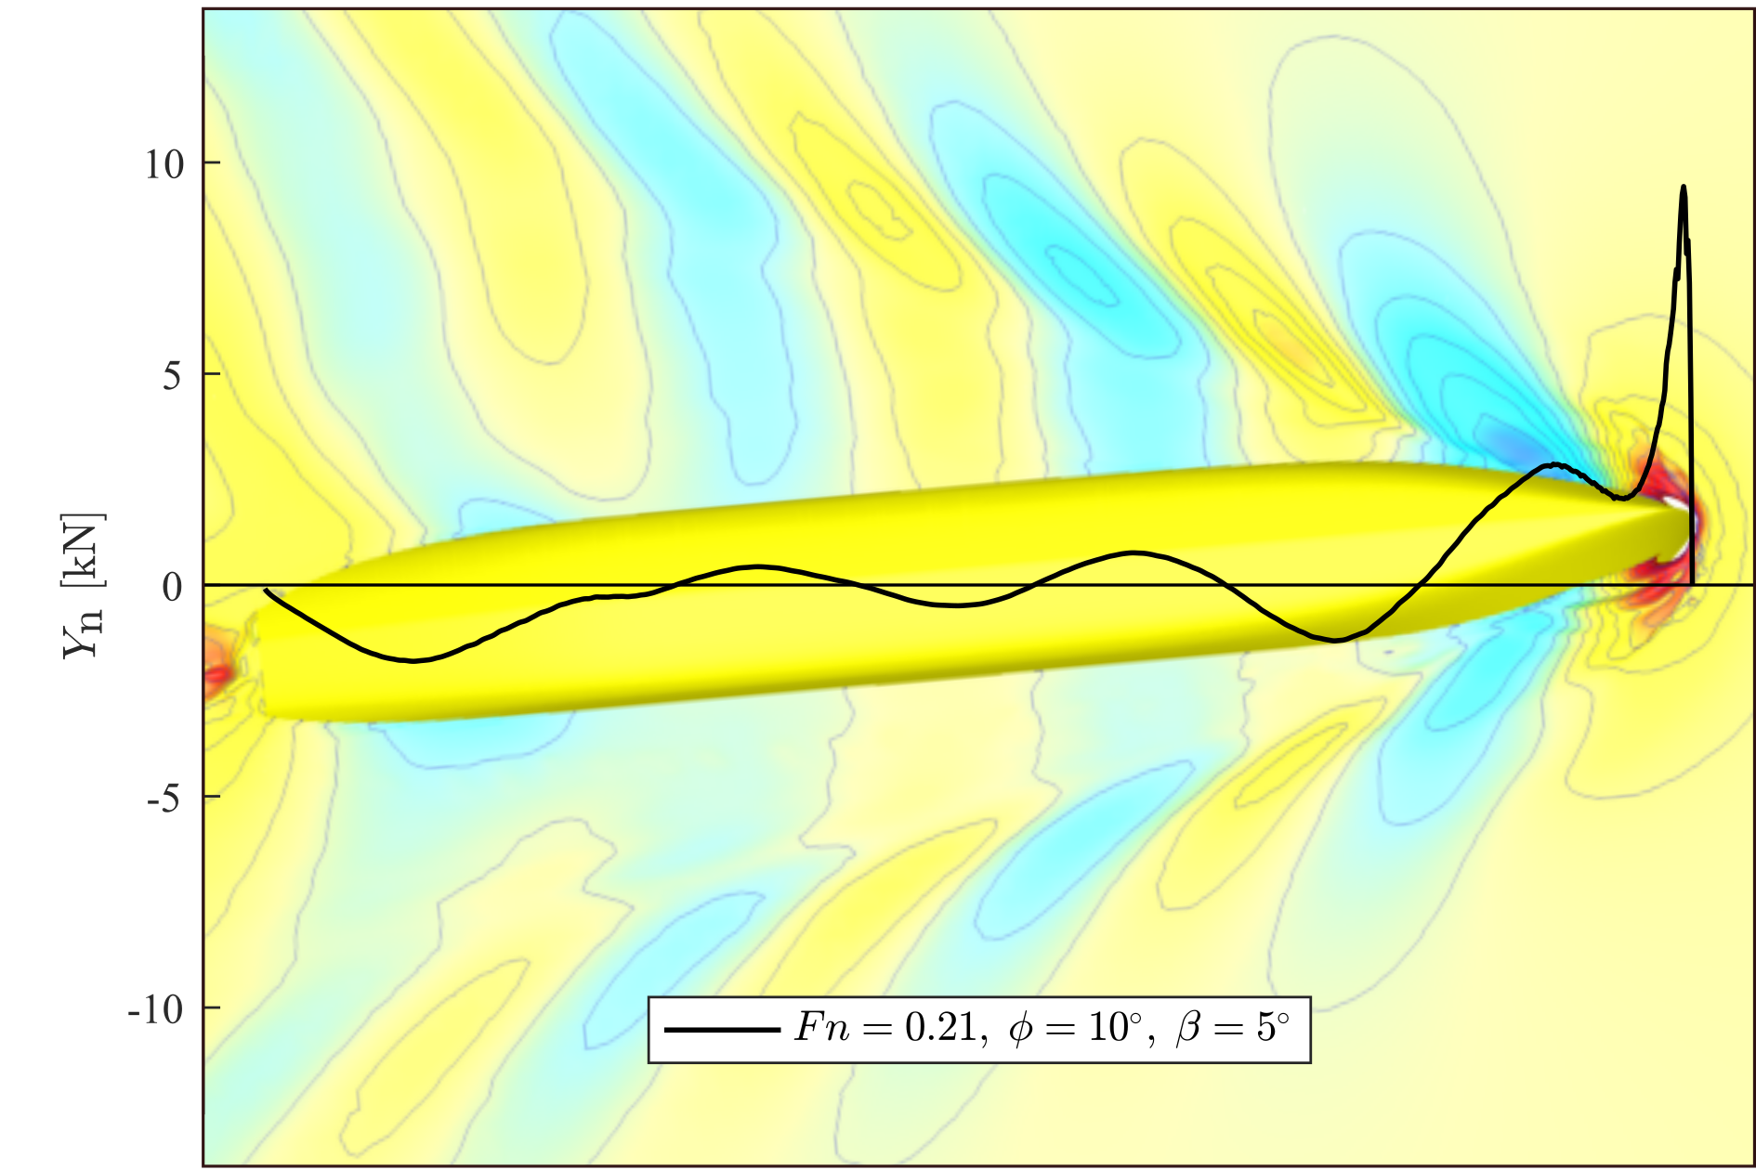
\includegraphics[width=\columnwidth]{images/hull1.png}  %assumes jpg extension
\caption{Fundamental diagram }
\label{fig:hull1}
\end{figure}

\subsection{Numerical modeling with machine learning}

Machine learning is a generic term that covers a broad range of analytical processes including linear regression. Machine learning uses datasets to train software to recognize patterns or predict outcomes by updating parameters within an algorithm that minimizes the error associated with the data. The error could be the difference between the expected output versus the calculated output or simply be the shortest distance between a set of point. The most common type of machine learning algorthims use supervised learning (SL) in which input data is labeled with the expected output. The algorithm, or network, is repeated trained with the input data until the output error is small enough.

The basic unit of machine learning is a node as shown in  Figure \ref{fig:node}.

The canonical FFNN model consists of an input layer, a hidden layer and an output layer. Each layer is constructed from interlinked nodes that generates a value (usually between -1 and 1 or 0 and 1). The individual node model is shown in Figure \ref{fig:node}. \\

\begin{figure}[]
\centering
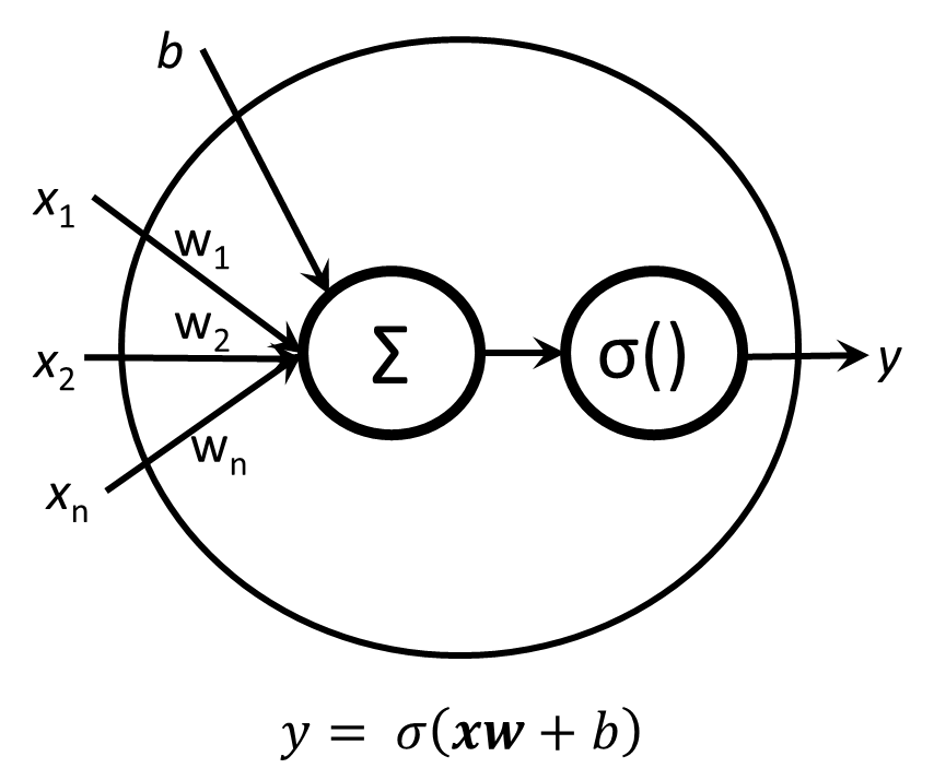
\includegraphics[width=\columnwidth]{images/node.png}  %assumes jpg extension
\caption{Basic node used in most machine learning architectures }
\label{fig:node}
\end{figure}
%
The node is based on the biologial neuron, where dendrites bring in sensory information in the form of bioelectric impulses until the neuron activates and sends another signal through its outputs. The machine learning node is similar to an individual neuron in that it also sums the weighted inputs of the previous layer, sometimes with a bias, and transforms the combined sum with a non-linear activation function, $\sigma$ before producing an output that becomes the input to other nodes or an output itself. The node  equation is given by

\begin{equation}
\label{eq:perceptron}
y= \sigma(wx+b)
\end{equation}
\noindent
where $w$ is an array of weights for the connections between the previous layer and the current layer, $x$ is a vector of input values from the previous layer, and $b$ is an optional bias value. Common activation functions include the sigmoid, tanh, and relu functions. A general property for activation functions is that they normalize the output and have a continuous first order derivative that can be used during the training process \cite{Goodfellow2016}. 

When many, or thousands, of nodes are used in a machine learning architecture, they become an artificial neural network (ANN). Because of the complex interconnections and nonlinear activation functions, ANNs have been successfully used to approximate complex functions and are often called ''universal approximators'' \cite{Sifaoui2008, Sonoda2017}. 

The basic ANN is a feed-forward neural network (FFNN) as shown in Figure \ref{fig:ffnn}. It includes an input layer that takes the input data features and distributes it to hidden layers for processing. The hidden layers due the bulk of the ANN calculations because of the interconnections between nodes. Each interconnection has a weight that can be updated or turned off. An output layer converts the final calculations into a binary category or a continuous value that may require further re-mapping.

\begin{figure}[]
\centering
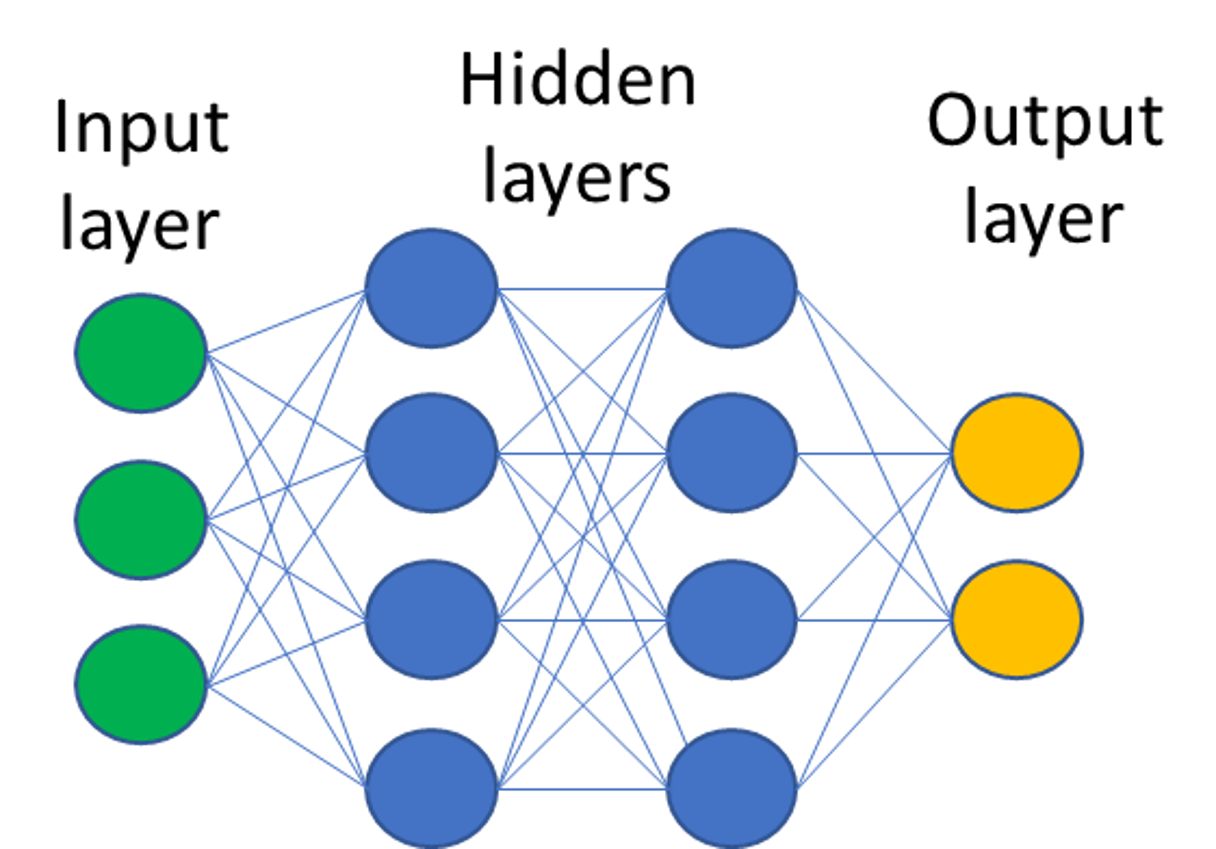
\includegraphics[width=\columnwidth]{images/ffnn.png}  %assumes jpg extension
\caption{Feed-forward neural network architecture}
\label{fig:ffnn}
\end{figure}
%

\begin{algorithm}
\caption{Calculate number of vehicles in 1000 m}
\label{alg:vehcount}
\begin{algorithmic}
\State $i=0$
\State $TotalDistance=0$
\While {$TotalDistance <$ 1000 m}
\State $VehicleClass_{i} = RAND(Class)$
\State $(l_{s})_{i} = RAND(Length(VehicleClass_{i}))$
\State $(\delta_{s})_{i} = RAND(\delta_{s})$
\State $(x_{s})_{i} =  (l_{s})_{i} + (\delta_{s})_{i}$
\State $TotalDistance = TotalDistance + (x_{s})_{i}$
\State $i = i + 1$
\EndWhile
\State $n = i$
\end{algorithmic}
\end{algorithm}

The benefits of using ANNs include not requiring \textit{a priori} assumptions of the data used for training and not requiring weighting of initial inputs \cite{Gardner1998}. In practice, dimensionality reduction is often used to remove inputs to the model that are not independent and identically distributed (IID) or offer little influence to the overall training. 

Training of ANNs use gradient-based optimization to update the weights that interconnect the nodes. Through a series of back propagation, the weights are individually modified in an iterative process. The training data is then run through the network again in order to measure the error again. Each complete cycle of training is called an epoch. There is no ''one-size-fits-all'' architecture and a key challenge of using machine learning tools is selecting an appropriate architecture based on the datasets available and the desired output \cite{Wolpert1997}.

This research uses datasets generated from RANS-CFD simulations on 61 different hull designs under various conditions defined by Froude number (Fn), leeway ($\beta$), and heel angle ($\phi$) to train multi-layer neural networks to simulate results in order to interpolate component forces under scenarios outside of the training set provided. 

%------------------------------------------------

 
\section{METHODOLOGY}

A multi layer FFNN was selected to model the RANS-CFD results. A total set of 1,567 different RANS-CFD runs were prepared and executed over the period of 2016 and 2019 using the XXX package. 

\subsection{Preparation of training data}

Training data set preparations vary based on the desired output the model is trained for. Because the RANS-CFD model assumed a steady-state output and ignored transient conditions, a non-sequential (non-Bayesian) sampling of training data could be used. Data sets are sampled randomly without replacement and fed to the FFNN along with the expected outputs. After shuffling the input observations, 70\% of the entire set was used for training while the remaining 30\% was reserved for testing the trained model.

Each input data observation included vehicle hull parameters as well as sailing performance parameters. Vessel sailing performance were summarized as a function of Froude number (Fn), leeway ($\beta$), and heel angle ($\phi$). The ranges of the different scenarios are shown in Table \ref{tab:parameters}.

\begin{table}[]
\centering
\caption{Initial parameters used to generate RANS-CFD model results}
\label{tab:parameters}
\begin{tabular}{@{}cc@{}}
\toprule
\textbf{Parameter} & \textbf{Values} \\ \midrule
Froud Number & 0.126, 0.168, 0.21 \\
Leeway ($\beta$) & 0, 3, 4, 5, 6, 7, 9 (deg) \\
Heel ($\phi$) & 0, 10, 20 (deg) \\ \bottomrule
\end{tabular}
\end{table}

The 61 different hulls were characterized using the parameters shown in Table \ref{tab:hull_parameters}.

\begin{table}[]
\centering
\caption{Hull descriptive parameters and ranges}
\label{tab:hull_parameters}
\begin{tabular}{@{}ccc@{}}
\toprule
\textbf{Parameter} & \textbf{Min Value} & \textbf{Max Value} \\ \midrule
C$_{p}$ & 0.549 & 0.840 \\
C$_{b}$ & 0.493 & 0.827 \\
C$_{m}$ & 0.787 & 0.988 \\
L/B & 5.998 & 8.444 \\
B/T & 2.156 & 3.538 \\
T/L & 0.042 & 0.061 \\
L/vol\textasciicircum{}1/3 & 5.769 & 6.473 \\
C$_{wp}$ & 0.747 & 0.925 \\
A$_{wp}$S$_{w}$ & 0.578 & 0.752 \\
R$_{b}$/T & 0.280 & 2.238 \\
Deadrise & 0.000 & 14.000 \\ \bottomrule
\end{tabular}
\end{table}

Data was normalized to a range of 0 and 1 using scaling methods. For parameters using degrees, the numbers were converted to sine and cosine components. 

\subsection{Model architecture}
Selection of hyperparameters for the FFNN were based on rule of thumbs and experience. Generally, final parameters are selected by iteratively training the model and finding the combinations that represent the best performance \cite{Freeman2018}. The parameters used for the model are shown in Table \ref{tab:network_parameters}.

\begin{table}[]
\centering
\caption{Network hyperparameters used to build the feed forward neural network}
\label{tab:network_parameters}
\resizebox{\columnwidth}{!}{%
\begin{tabular}{@{}cc@{}}
\toprule
\textbf{Neural Network Parameter} & \textbf{Value} \\ \midrule
Hidden layers & 2 \\
Hidden layer nodes & 30 \\
Input and hidden layer activation function & sigmoid \\
Output activation function & tanh \\
learning rate ($\alpha_{lr}$) & 0.002 \\
Optimizer & Nesterov Adam \\
Loss Function & Mean Square Error \\
Dropout & 0.2 \\
Batches & 100 \\ \bottomrule
\end{tabular}
}
\end{table}


\section{RESULTS}

\section{DISCUSSION}




\section{CONCLUSIONS}

The main body of the text must end with the conclusions of the paper.

\section{ACKNOWLEDGEMENTS}

Short acknowledgements may be added.


\bibliography{dwas-bib}

\section{AUTHORS BIOGRAPHY}

Brief biographies are required for all authors e.g.:

\textbf{B. Freeman}is a Senior Project Manager at Lakes Software.  He is responsible for researching new machine learning applications and conducting complex air dispersion modeling using CFD methods.  He holds a Ph.D. in Environmental Engineering from the University of Guelph, Canada. His current interests includes deep learning analysis of spatio-temporal events and multi-sensor integration.

\textbf{N. van der Kolk} holds the current position of [job title] at [name of organisation].  He is responsible for [brief job description].  His previous experience includes [previous experience relevant to the paper], etc.

% That's all folks!
\end{document}
